% ============================================================================================
% BAB III ANALISIS MASALAH
% Pembagian subbab tidak rigid dan dapat bervariasi. Bab ini minimal berisi analisis kebutuhan
% fungsional dan nonfungsional, analisis berbagai alternatif solusi yang dapat ditawarkan, dan
% metode pemilihan solusi yang diusulkan.
% ============================================================================================
\chapter{ANALISIS MASALAH}
\label{chap:analisis-masalah}
\section{Analisis Kondisi Saat Ini}

Dalam merancang mekanisme rekomendasi \textit{people-to-people} pada aplikasi yang akan dibuat, penting untuk memahami terlebih dahulu kondisi faktual terkait bagaimana mahasiswa saat ini menemukan rekan kolaborasi serta tantangan yang mereka hadapi. Analisis kondisi ini disusun berdasarkan hasil survei yang melibatkan 19 mahasiswa dari berbagai semester dan program studi. Hasil survei memberikan gambaran yang jelas mengenai pola perilaku, kendala, serta kebutuhan mahasiswa dalam proses pencarian partner kolaborasi.

\begin{figure}[h] % pilihan opsi yang disarankan: t = top, b = bottom, h = here
	\centering
  \captionsetup{justification=centering}
    	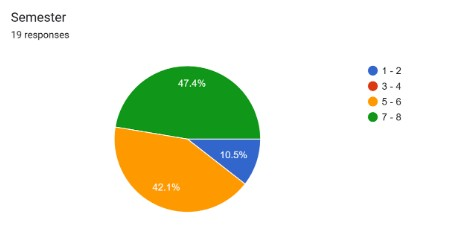
\includegraphics[width=0.7\textwidth]{image/31.jpg}
	\caption{Distribusi semester responden}
	\label{gambar:31}
\end{figure}

Distribusi semester responden dapat dilihat pada Gambar III.1. Sebagian besar responden berada pada semester 5–6 (42,1\%) dan semester 7–8 (47,4\%), sedangkan hanya sebagian kecil berada pada semester awal (10,5\%). Kondisi ini menunjukkan bahwa mayoritas responden merupakan mahasiswa tingkat menengah dan akhir, yaitu kelompok yang paling sering terlibat dalam kegiatan kolaboratif seperti lomba, proyek akademik, magang, dan kegiatan organisasi. Oleh karena itu, respon mereka relevan sebagai representasi kebutuhan pengguna aplikasi yang akan dikembangkan.

\begin{figure}[h] % pilihan opsi yang disarankan: t = top, b = bottom, h = here
	\centering
  \captionsetup{justification=centering}
    	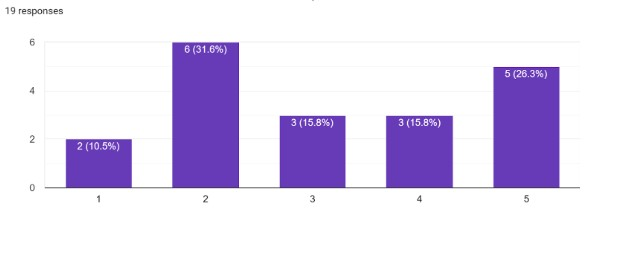
\includegraphics[width=0.7\textwidth]{image/32.jpg}
	\caption{Tingkat partisipasi mahasiswa dalam kegiatan kolaboratif}
	\label{gambar:32}
\end{figure}

Berdasarkan Gambar III.2, tingkat partisipasi mahasiswa dalam kegiatan kolaboratif bervariasi, namun mayoritas berada pada kategori rendah hingga sedang. Sebanyak 31,6\% responden memilih nilai 2, sedangkan 26,3\% memilih nilai 5. Perbedaan ini menunjukkan bahwa meskipun sebagian mahasiswa aktif, sebagian lainnya memiliki keterlibatan yang tidak konsisten dalam aktivitas kolaboratif.

Temuan ini dapat mengindikasikan adanya hambatan tertentu yang membuat mahasiswa tidak aktif mengikuti kegiatan kolaboratif secara rutin, baik dari sisi akses informasi, kesulitan menemukan partner, maupun kurangnya sistem yang memfasilitasi proses pencarian tim.

\begin{figure}[h] % pilihan opsi yang disarankan: t = top, b = bottom, h = here
	\centering
  \captionsetup{justification=centering}
    	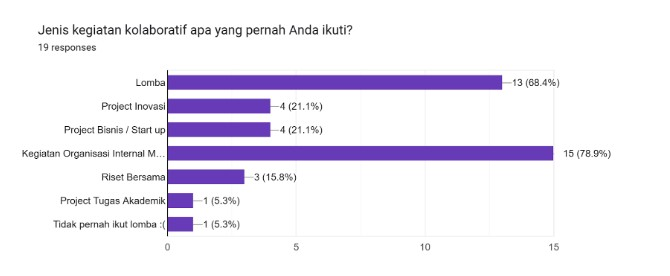
\includegraphics[width=0.7\textwidth]{image/33.jpg}
	\caption{Jenis kegiatan yang paling banyak diikuti}
	\label{gambar:33}
\end{figure}

Pada Gambar III.3, jenis kegiatan yang paling banyak diikuti adalah kegiatan organisasi internal (78,9\%) dan lomba (68,4\%). Aktivitas lain seperti projek inovasi, project bisnis/startup, dan riset bersama berada pada kisaran 15–21\%. Hanya 5,3\% responden yang menyatakan tidak pernah mengikuti kegiatan kolaboratif.

Distribusi ini menunjukkan bahwa ekosistem kolaborasi mahasiswa cukup beragam, namun bentuk kolaborasi yang bersifat kompetitif dan organisasi masih mendominasi. Kondisi ini menguatkan kebutuhan akan sistem pencarian partner yang dapat membantu mahasiswa memilih rekan yang paling sesuai untuk konteks kegiatan yang berbeda-beda.

\begin{figure}[h] % pilihan opsi yang disarankan: t = top, b = bottom, h = here
	\centering
  \captionsetup{justification=centering}
    	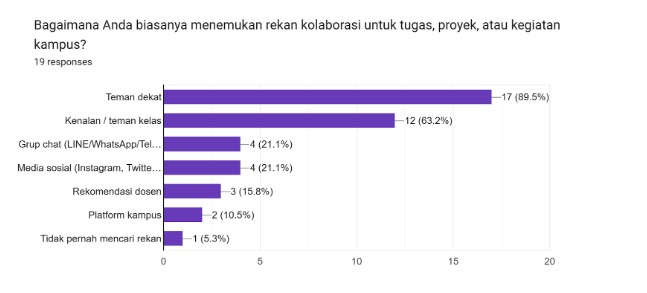
\includegraphics[width=0.7\textwidth]{image/34.jpg}
	\caption{Jalur menemukan rekan kolaborasi}
	\label{gambar:34}
\end{figure}

Gambar III.4 menunjukkan bahwa sebagian besar mahasiswa menemukan rekan kolaborasi melalui teman dekat (89,5\%) dan kenalan atau teman kelas (63,2\%). Kanal lain seperti grup chat, media sosial, atau rekomendasi dosen hanya digunakan sekitar 15–21\%.

Menariknya, hanya 10,5\% responden yang pernah menggunakan platform kampus, dan tidak ada responden yang mengandalkan platform khusus untuk menemukan partner. Temuan ini menegaskan bahwa proses pencarian partner masih sangat bergantung pada jejaring sosial pribadi, yang memiliki keterbatasan besar, seperti lingkaran pertemanan yang sempit, kurangnya keberagaman profil, dan tidak adanya cara untuk menilai kecocokan secara objektif.

\begin{figure}[h] % pilihan opsi yang disarankan: t = top, b = bottom, h = here
	\centering
  \captionsetup{justification=centering}
    	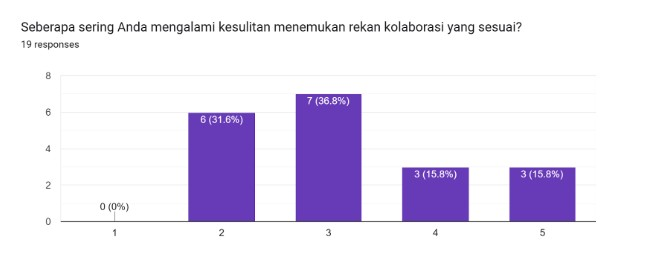
\includegraphics[width=0.7\textwidth]{image/35.jpg}
	\caption{Tingkat kesulitan menemukan rekan kolaborasi}
	\label{gambar:35}
\end{figure}

Pada Gambar III.5, mayoritas responden memilih tingkat kesulitan 2 (31,6\%) dan 3 (36,8\%). Sebagian lainnya menyatakan kesulitan tinggi (kategori 4 dan 5) sebanyak 31,6\%. Tidak ada responden yang menyatakan tidak mengalami kesulitan sama sekali. Data ini menunjukkan bahwa proses menemukan partner yang sesuai bukanlah hal yang mudah bagi mahasiswa. Kesulitan ini dapat terjadi karena kurangnya informasi mengenai profil calon rekan, ketidaksesuaian minat atau skill, maupun keterbatasan jaringan pertemanan.

\begin{figure}[h] % pilihan opsi yang disarankan: t = top, b = bottom, h = here
	\centering
  \captionsetup{justification=centering}
    	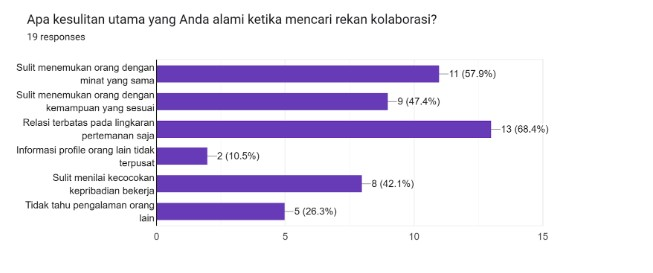
\includegraphics[width=0.7\textwidth]{image/36.jpg}
	\caption{Tantangan dalam mencari rekan kolaborasi}
	\label{gambar:36}
\end{figure}

Gambar III.6 menunjukkan tiga masalah terbesar yang dialami mahasiswa, seperti relasi terbatas pada lingkaran pertemanan (68,4\%), sulit menemukan orang dengan minat yang sama (57,9\%), dan sulit menemukan orang dengan kemampuan yang sesuai (47,4\%). Masalah lain yang juga muncul adalah sulit menilai kepribadian atau gaya kerja (42,1\%) serta tidak mengetahui pengalaman calon partner (26,3\%).Temuan ini semakin memperkuat bahwa hambatan terbesar mahasiswa bukan hanya kurangnya informasi, tetapi juga ketidakmampuan mereka menilai kecocokan partner secara objektif.

Berdasarkan seluruh data survei, dapat disimpulkan bahwa kondisi mahasiswa saat ini sangat bergantung pada jaringan sosial pribadi dalam mencari partner, tidak memiliki akses ke platform yang terpusat dan sistematis untuk menemukan rekan kolaborasi yang sesuai, dan mengalami kesulitan dalam menilai kecocokan partner berdasarkan minat, skill, pengalaman, dan gaya kerja. Oleh karena itu, dibutuhkan sistem yang dapat membantu menampilkan profil mahasiswa lain secara relevan dan terarah. 

\section{Analisis Kebutuhan}
Analisis kebutuhan pengguna dilakukan untuk memahami apa yang sebenarnya diperlukan mahasiswa dalam proses pencarian kegiatan kolaboratif. Analisis kebutuhan ini dilakukan berdasarkan hasil survei serta interpretasi terhadap perilaku dan hambatan yang dialami pengguna. Pendekatan ini penting agar solusi yang dikembangkan tidak hanya menjawab permasalahan secara umum, tetapi mampu mengakomodasi kebutuhan nyata mahasiswa dalam konteks yang lebih spesifik.

\subsection{Identifikasi Masalah pengguna}
Untuk mengidentifikasi permasalahan utama yang dialami mahasiswa dalam proses mencari rekan kolaborasi, dilakukan analisis terhadap hasil survei yang menggali hambatan, persepsi, serta faktor-faktor penting yang dipertimbangkan mahasiswa dalam menentukan kecocokan partner. Hasil analisis ini menjadi dasar penentuan kebutuhan pengguna dan menjadi pijakan bagi perancangan sistem rekomendasi yang relevan.

Berdasarkan data pada Gambar III.6, terlihat bahwa salah satu hambatan terbesar yang dialami mahasiswa adalah relasi yang terbatas pada lingkaran pertemanan (68,4%). Kondisi ini menunjukkan bahwa mahasiswa cenderung hanya mengenal calon partner dari jaringan sosial yang sempit sehingga peluang menemukan rekan yang cocok menjadi terbatas. Ketergantungan pada jejaring informal membuat proses pencarian partner menjadi tidak efisien, kurang beragam, dan menyulitkan mahasiswa untuk mengeksplorasi potensi kolaborasi yang lebih luas.

Selain itu, mahasiswa juga mengaku mengalami kesulitan dalam menemukan rekan dengan minat yang sama (57,9\%) dan kemampuan yang sesuai (47,4\%). Kesulitan ini mengindikasikan tidak tersedianya informasi profil yang cukup untuk menilai kecocokan antar mahasiswa. Tanpa data yang struktural mengenai minat, skill, atau pengalaman, mahasiswa kesulitan menentukan apakah seseorang benar-benar cocok menjadi partner dalam proyek tertentu.

Aspek lain yang juga signifikan adalah kesulitan dalam menilai kecocokan gaya kerja atau kepribadian (42,1\%). Meskipun faktor-faktor ini sangat penting dalam kolaborasi, mahasiswa tidak memiliki mekanisme yang dapat membantu mereka memahami preferensi kerja atau karakter calon partner. Kondisi ini menyebabkan tingginya risiko ketidaksesuaian dalam bekerja sama, misalnya perbedaan ritme kerja, komitmen, atau ekspektasi terhadap pembagian tugas.

Kesulitan lain seperti tidak mengetahui pengalaman orang lain (26,3\%) serta informasi profil yang tidak terpusat (10,5\%) semakin memperjelas bahwa mahasiswa membutuhkan sistem yang dapat:
\begin{enumerate}
\item {menyediakan informasi profil yang lebih lengkap,} 
\item {menyajikan data tersebut secara terstruktur dan mudah dipahami, serta}
\item {mempermudah penilaian kecocokan antar mahasiswa.}
\end{enumerate}

Jika dilihat secara keseluruhan, hasil survei menunjukkan bahwa mahasiswa menghadapi tiga kelompok masalah utama dalam proses pencarian partner kolaborasi:
\begin{enumerate}
\item {Akses informasi yang tidak terpusat, sehingga mahasiswa bergantung pada media informal dan jaringan yang sempit.} 
\item {Kesulitan menilai kecocokan partner, terutama terkait minat, kemampuan, pengalaman, gaya kerja, dan kepribadian.}
\item {Kurangnya mekanisme rekomendasi yang membantu mahasiswa menemukan partner yang relevan secara cepat dan akurat.}
\end{enumerate}

Ketiga masalah ini mempertegas perlunya pengembangan fitur \textit{People-to-People} pada platform yang akan dibuat, yang diharapkan mampu memberikan rekomendasi rekan kolaborasi secara terarah berdasarkan kesesuaian profil, preferensi, dan kebutuhan pengguna.

\subsection{Kebutuhan Fungsional}
Kebutuhan fungsional merupakan fungsi-fungsi inti yang harus disediakan oleh sistem agar mampu menjawab permasalahan yang telah diidentifikasi sebelumnya. Fungsi-fungsi ini dirancang berdasarkan hasil analisis masalah pengguna, preferensi mahasiswa, serta atribut-atribut yang dianggap penting untuk menentukan kecocokan partner. Kebutuhan fungsional berikut menjadi dasar pengembangan mekanisme rekomendasi dan fitur \textit{People-to-People} pada aplikasi yang akan dikembangkan.

\begin{longtable}{@{\extracolsep{\fill}} p{1.2cm} p{4cm} p{9cm}}
\caption{Kebutuhan Fungsional Sistem}\label{tbl:kebutuhan-fungsional} \\
\toprule
\textbf{Kode} & \textbf{Kebutuhan Fungsional} & \textbf{Deskripsi} \\
\midrule
\endfirsthead

\caption [] {Kebutuhan Fungsional Sistem (lanjutan)} \\
\toprule
\textbf{Kode} & \textbf{Kebutuhan Fungsional} & \textbf{Deskripsi} \\
\midrule
\endhead

\midrule
\multicolumn{3}{r}{\textit{Bersambung ke halaman berikutnya}} \\
\bottomrule
\endfoot

\bottomrule
\endlastfoot

% === Data Tabel ===
F01 & Pengelolaan profil pengguna &
Sistem harus mampu mengumpulkan, menyimpan, dan memperbarui data profil mahasiswa, termasuk minat, skill, pengalaman proyek, gaya kerja, dan ketersediaan waktu. \\

F02 & Pembaruan preferensi pengguna &
Pengguna harus dapat memperbarui preferensi mereka sewaktu-waktu agar sistem dapat menampilkan rekomendasi yang tetap relevan. \\

F03 & Pengelolaan data atribut kecocokan &
Sistem harus menyediakan struktur data untuk menyimpan atribut penting dalam penilaian kecocokan seperti minat, skill, \textit{tools/tech stack}, pengalaman, motivasi, dan kepribadian/gaya kerja. \\

F04 & Mekanisme pencocokan &
Sistem harus memiliki mekanisme untuk menghitung skor kecocokan antar pengguna berdasarkan bobot atribut yang relevan. Mekanisme ini menjadi inti rekomendasi. \\

F05 & Penyajian hasil pencocokan &
Sistem harus dapat menampilkan daftar mahasiswa lain dalam bentuk \textit{feed} rekomendasi yang diurutkan berdasarkan tingkat kecocokan. \\

F06 & Tampilan detail profil rekan &
Sistem harus menyediakan halaman profil lengkap yang memungkinkan pengguna melihat informasi penting calon partner secara terstruktur. \\

F07 & Interaksi dasar antar pengguna &
Sistem menyediakan fitur dasar seperti \textit{save profile}, \textit{express interest}, dan \textit{connect request} agar pengguna dapat menindaklanjuti rekomendasi yang diberikan. \\

\end{longtable}

\subsection{Kebutuhan Non-Fungsional}
Kebutuhan non-fungsional merupakan aspek kualitas yang harus dipenuhi oleh sistem agar dapat digunakan secara nyaman, efisien, aman, dan dapat diandalkan oleh pengguna. Dalam konteks pengembangan fitur \textit{People-to-People} pada platform yang akan dikembangkan, kebutuhan non-fungsional ini penting untuk memastikan bahwa pengalaman pengguna konsisten dan mendukung tujuan pencarian partner secara efektif.

\begin{longtable}{@{\extracolsep{\fill}} p{1.5cm} p{4cm} p{9cm}}
\caption{Kebutuhan Non-Fungsional Sistem}\label{tbl:nonfunctional} \\
\toprule
\textbf{Kode} & \textbf{Kebutuhan Non-Fungsional} & \textbf{Deskripsi} \\
\midrule
\endfirsthead

\caption[]{Kebutuhan Non-Fungsional Sistem (lanjutan)} \\
\toprule
\textbf{Kode} & \textbf{Kebutuhan Non-Fungsional} & \textbf{Deskripsi} \\
\midrule
\endhead

\midrule
\multicolumn{3}{r}{\textit{Bersambung ke halaman berikutnya}} \\
\bottomrule
\endfoot

\bottomrule
\endlastfoot

% ----------- DATA TABEL ----------------

NF01 & \textit{Usability} &
Sistem harus mudah digunakan, memiliki antarmuka yang intuitif, dan dapat dipahami oleh mahasiswa tanpa pelatihan khusus. \\

NF02 & \textit{Performance} &
Sistem harus dapat menampilkan hasil pencocokan atau rekomendasi dalam waktu yang cepat dan responsif. \\

NF03 & \textit{Reliability} &
Sistem harus memberikan hasil yang konsisten dan stabil untuk input yang sama. \\

NF04 & \textit{Privacy} &
Sistem harus menjamin keamanan data pengguna dan melindungi informasi sensitif. \\

NF05 & \textit{Security} &
Sistem harus aman dari berbagai ancaman dan serangan siber. \\

\end{longtable}

\section{Analisis Pemilihan Solusi}
Analisis pemilihan solusi pada subbab ini tidak berfokus pada penentuan metode pencocokan, karena metode yang digunakan dalam tugas akhir ini telah ditetapkan berdasarkan kajian literatur pada Bab II yang menunjukkan bahwa metode tersebut paling sesuai untuk konteks \textit{people-to-people recommendation} berbasis atribut multidimensi mahasiswa.

Oleh karena itu, analisis pemilihan solusi pada bagian ini difokuskan pada pemilihan platform implementasi yang paling tepat untuk menjalankan mekanisme rekomendasi tersebut. Pemilihan platform penting untuk memastikan bahwa sistem dapat diakses, digunakan, dan dikembangkan secara efektif sesuai dengan keterbatasan proyek Tugas Akhir serta kebutuhan mahasiswa sebagai pengguna utama.

\subsection{Alternatif Solusi}
Berbagai bentuk solusi dapat dipertimbangkan dalam mengatasi permasalahan mahasiswa yang kesulitan mencari kegiatan kolaboratif. Berikut merupakan empat alternatif solusi yang dianalisis sebelum menentukan pendekatan yang paling tepat.
\begin{enumerate}
\item {\textit{Mobile Application}} 
Aplikasi mobile menjadi salah satu alternatif solusi untuk menghubungkan mahasiswa dengan berbagai mahasiswa lainnya melalui platform yang dapat diakses langsung dari perangkat smartphone. \textit{Mobile app} menjadi wadah bagi mahasiswa dalam memperoleh informasi, pembaruan, dan akses terhadap layanan \textit{people to people} kapan saja dan di mana saja.
\item {\textit{Website Based Application}}
Aplikasi berbasis web merupakan alternatif yang paling fleksibel dan mudah diakses untuk mendukung proses pencocokan \textit{people to people}. Platform ini dapat digunakan tanpa instalasi, dapat diakses melalui berbagai perangkat, dan lebih mudah dikembangkan secara bertahap. 
\item {\textit{Social Media Channel}}
Pemanfaatan kanal media sosial menjadi alternatif solusi yang bersifat praktis dan cepat diterapkan untuk membantu mahasiswa menemukan rekan yang cocok. Melalui grup, channel, atau akun khusus, informasi mengenai proyek dapat disebarkan secara luas dan instan. Pendekatan ini relevan dengan kebiasaan mahasiswa yang aktif menggunakan platform komunikasi tersebut.
\item {\textit{Digital Board}}
Digital board merupakan bentuk solusi yang menyediakan tampilan informasi proyek secara terpusat dan terorganisasi. Platform ini dapat berupa papan pengumuman digital, dashboard sederhana, atau laman informasi yang diperbarui secara berkala. 
\end{enumerate}

\subsection{Analisis Penentuan Solusi}
Dalam menentukan solusi yang paling tepat untuk mengatasi masalah pencarian proyek mahasiswa, diperlukan metode yang mampu mengevaluasi beberapa alternatif secara sistematis dan objektif. \textit{Weighted Scoring Model} (WSM) merupakan metode penilaian multi kriteria yang digunakan untuk membandingkan beberapa alternatif solusi berdasarkan sejumlah kriteria yang memiliki bobot atau tingkat kepentingan tertentu. Menurut \textcite{MarketSegmentationAssessment2022}, WSM bekerja secara efektif untuk kasus pengambilan keputusan yang bersifat satu dimensi, karena setiap alternatif dievaluasi secara numerik terhadap masing-masing kriteria, lalu dihitung skor totalnya berdasarkan pembobotan. Metode ini menghasilkan proses penilaian yang transparan, mudah direplikasi, serta sesuai untuk pengambilan keputusan yang membutuhkan struktur evaluasi sederhana namun objektif. 

\textcite{MarketSegmentationAssessment2022} menjelaskan bahwa proses pemilihan solusi dilakukan melalui beberapa langkah. Tahapan pertama adalah menentukan alternatif solusi, yang disajikan pada Tabel sekian.
\begin{table}[h]
\centering
\begin{tabular}{|p{2cm}|p{10cm}|}
\hline
\textbf{Kode} & \textbf{Alternatif Solusi} \\
\hline
A1 & \textit{Mobile Application} \\
\hline
A2 & \textit{Website Based Application} \\
\hline
A3 & \textit{Social Media Channel} \\
\hline
A4 & \textit{Digital Board} \\
\hline
\end{tabular}
\caption{Daftar Alternatif Solusi}
\label{tbl:alternatif-solusi}
\end{table}

Setelah menentukan alternatif solusi, tahapan selanjutnya adalah menetapkan kriteria evaluasi yang disajikan pada Tabel sekian.
\begin{table}[h]
\centering
\begin{tabular}{|p{2cm}|p{10cm}|}
\hline
\textbf{Kode} & \textbf{Kriteria Evaluasi} \\
\hline
K1 & Kemampuan menyelesaikan masalah pengguna \\
\hline
K2 & Fleksibilitas \\
\hline
K3 & Kemudahan penggunaan \\
\hline
K4 & Kelayakan implementasi \\
\hline
\end{tabular}
\caption{Kriteria Evaluasi Alternatif Solusi}
\label{tbl:kriteria-evaluasi}
\end{table}

Setelah kriteria evaluasi ditetapkan, langkah berikutnya dalam proses \textit{Weighted Scoring Method} adalah menetapkan bobot untuk setiap kriteria. Pada tugas akhir ini digunakan pendekatan equal weighting, yaitu seluruh kriteria diberikan bobot yang sama. Krishna Kumar et al. (2022) menjelaskan bahwa seluruh kriteria dianggap memiliki tingkat kepentingan yang setara sehingga masing-masing diberi bobot identik. Selanjutnya adalah memberikan nilai pada setiap alternatif. Nilai diberikan menggunakan skala 1–5 sesuai tingkat pemenuhan kriteria yang disajikan pada tabel sekian.
\begin{table}[h]
\centering
\begin{tabular}{|p{2cm}|p{2cm}|p{2cm}|p{2cm}|p{2cm}|}
\hline
\textbf{Alternatif} & \textbf{K1} & \textbf{K2} & \textbf{K3} & \textbf{K4} \\
\hline
A1 & 4 & 2 & 3 & 2 \\
\hline
A2 & 5 & 4 & 4 & 3 \\
\hline
A3 & 2 & 3 & 4 & 5 \\
\hline
A4 & 1 & 3 & 4 & 4 \\
\hline
\end{tabular}
\caption{Penilaian Alternatif terhadap Kriteria Evaluasi}
\label{tbl:penilaian-alternatif}
\end{table}

Tahapan berikutnya adalah melakukan perhitungan skor komposit untuk menentukan solusi terbaik. Karena setiap kriteria menggunakan skala penilaian yang sama dan bobot yang digunakan adalah \textit{equal weighting}, proses normalisasi tidak diperlukan. Nilai pada masing-masing kriteria kemudian dijumlahkan untuk memperoleh total skor setiap alternatif, sebelum dikalikan dengan bobot kriteria yang identik, yaitu 0,25 untuk masing-masing kriteria. 
\begin{table}[h]
\centering
\begin{tabular}{|p{2cm}|p{3cm}|p{3cm}|p{2cm}|}
\hline
\textbf{Alternatif} & \textbf{Total Nilai} & \textbf{Skor Akhir} & \textbf{Peringkat} \\
\hline
A1 & 11 & 2,75 & 4 \\
\hline
\textbf{A2} & \textbf{16} & \textbf{4,00} & \textbf{1} \\
\hline
A3 & 14 & 3,50 & 2 \\
\hline
A4 & 12 & 3,00 & 3 \\
\hline
\end{tabular}
\caption{Hasil Perhitungan Weighted Scoring Method}
\label{tbl:wsm-hasil}
\end{table}

Berdasarkan tabel sekian Solusi alternatif kedua atau \textit{Website Based Application}  memperoleh skor tertinggi dengan nilai akhir 4.00. \textit{Website} unggul dalam kemampuan menyelesaikan masalah pengguna, fleksibilitas pengembangan, serta kemudahan penggunaan, sementara kompleksitas implementasinya tetap berada pada tingkat yang realistis untuk direalisasikan dalam konteks tugas akhir. Dengan demikian, \textit{Website Based Application} ditetapkan sebagai solusi terbaik untuk dikembangkan dalam tugas akhir ini.
